\chapter{Background}
\section{Image Formats}
\subsection{Open WSI Formats}
\subsubsection{Deep Zoom Images}
\section{Short Introduction to Neural Networks}

% https://www.doc.ic.ac.uk/~nd/surprise_96/journal/vol4/cs11/report.html#Introduction to neural networks

% http://natureofcode.com/book/chapter-10-neural-networks/

% http://ufldl.stanford.edu/tutorial/supervised/MultiLayerNeuralNetworks/

\section{Microservices}
The following section elaborates on the concept of \emph{Microservices} (MS)\nmc{MS}{Microservice}, defining what they are, listing their pros and cons, as well as explaining why this approach was chosen over a monolithic approach. A monolithic software solution is described by \cite{Lewis14} as follows:
\begin{quotation}
	"[...] a monolithic application [is] built as a single unit. Enterprise Applications are often built in three main parts: a client-side user interface (consisting of HTML pages and javascript running in a browser on the user's machine) a database (consisting of many tables inserted into a common, and usually relational, database management system), and a server-side application. The server-side application will handle HTTP requests, execute domain logic, retrieve and update data from the database, and select and populate HTML views to be sent to the browser. This server-side application is a monolith - a single logical executable. Any changes to the system involve building and deploying a new version of the server-side application."
\end{quotation}


\subsection{Definition}
MS are an interpretation of the Service Oriented Architecture. The concept is to separate one monolithic software construct into several smaller, modular pieces of software\cite{Wolff16}. As such, MS are a modularization concept. However, they differ from other such concepts, since MS are independent from each other. This is a trait, other modularization concepts usually lack\cite{Wolff16}. As a result, changes in one MS don't bring up the necessity of deploying the whole product cycle again, but just the one service. This can be achieved by turning each MS into an independent process with its own runtime\cite{Lewis14}.

This modularization creates an information barrier between different MS. Therefore, if MS need to share data or communicate with each other, light weight communication mechanisms must be established, such as a RESTful API\cite{Riggins15}.

Even though MS are more a concept than a specific architectural style, certain traits are usually shared between them\cite{Riggins15}. According to \cite{Riggins15} and \cite{Lewis14}, those are:

\begin{enumerate}[(a)]
	\item \textbf{Componentization as a Service:} bringing chosen components (e.g. external libraries) together to make a customized service
	\item \textbf{Organized Around Business Capabilities:} cross-functional teams, including the full range of skills required to achieve the MS goal
	\item \textbf{Products instead of Projects:} teams own a product over its full lifetime, not just for the remainder of a project
	\item \textbf{Smart Endpoints and Dumb Pipes:} each microservice is as decoupled as possible with its own domain logic
	\item \textbf{Decentralized Governance:} enabling developer choice to build on preferred languages for each component.
	\item \textbf{Decentralized Data Management:} having each microservice label and handle data differently
	\item \textbf{Infrastructure Automation:} including automated deployment up the pipeline
	\item \textbf{Design for Failure:} a consequence of using services as components, is that applications need to be designed so that they can tolerate the failure of single or multiple services
\end{enumerate}

Furthermore, \cite{Bugwadia15} defined 5 architectural constraints, which should help to develop a MS:

\begin{enumerate}[(1.)]
	\item \textbf{Elastic}\\
	The elasticity constraint describes the ability of a MS to scale up or down, without affecting the rest of the system. This can be realized in different ways. \cite{Bugwadia15} suggests to architect the system in such a fashion, that multiple stateless instances of each microservice can run, together with a mechanism for Service naming, registration, and discovery along with routing and load-balancing of requests.
	\item \textbf{Resilient}\\
	This constraint is referring to the before mentioned trait (h) - \emph{Design for Failure}. The failure of or an error in the execution of a MS must not impact other services in the system.
	\item \textbf{Composable}\\
	To avoid confusion, different MS in a system should have the same way of identifying, representing, and manipulating resources, describing the API schema and supported API operations.
	\item \textbf{Minimal}\\
	A MS should only perform one single business function, in which only semantically closely related components are needed.
	\item \textbf{Complete}\\
	A MS must offer a complete functionality, with minimal dependencies to other services. Without this constraint, services would be interconnected again, making it impossible to upgrade or scale individual services.
\end{enumerate}


\subsection{Advantages and Disadvantages}
% pros
One big advantage of this modularization is that each service can be written in a different programming language, using different frameworks and tools. Furthermore, each microservice can bring along its own support services and data storages. It is imperative for the concept of modularization, that each microservice has its own storage of which it is in charge of\cite{Wolff16}.

The small and focused nature of MS makes scaling, updates, general changes and the deploying process easier. Furthermore, smaller teams can work on smaller code bases, making the distribution of know how easier\cite{Riggins15}.

Another advantage is how well MS plays into the hands of agile, scrum and continuous software development processes, due to their previously discussed inherent traits.

% cons
The modularization of MS doesn't only yield advantages. Since each MS has its own, closed off data management\footnote{See 2.3.1(f) (\emph{Decentralized Data Management})}, interprocess communication becomes a necessity. This can lead to communicational overhead which has a negative impact on the overall performance of the system\cite{Wolff16}.

2.3.1(e) (\emph{Decentralized Governance}) can lead to compatibility issues, if different developer teams chose to use different technologies. Thus, more communication and social compatibility between teams is required. This can lead to an unstable system which makes the deployment of extensive workarounds necessary\cite{Riggins15}.

It often makes sense to share code inside a system to not replicate functionality which is already there and therefore increase the maintenance burden. The independent nature of MS can make that very difficult, since shared libraries must be build carefully and with the fact in mind, that different MS may use different technologies, possibly creating dependency conflicts.


\subsection{Conclusion}	
After consideration of the advantages and disadvantages of MS, the author decided in favor of using them. This is mainly due to the fact of working alone on the project, negating some of their inherent disadvantages:
\begin{itemize}
	\item Interprocess communication doesn't arise between the single stages of the process chain, since they have a set order\footnote{E.g. it wouldn't make sense trying extract a training sample without converting or annotating a WSI first.}
	\item Different technologies may be chosen for the single steps of the process chain, however, working alone on the project makes technological incompatibilities instantly visible
	\item The services shouldn't share functionality, therefore there should be no need for shared libraries
\end{itemize}
This makes the advantages outweight the disadvantages clearly:
\begin{itemize}
	\item different languages and technologies can be used for every single step of the process chain, making the choice of the most fitting tool possible
	\item WSIs take a heavy toll on memory and disk space due to their size; the use of MS allows each step of the chain to handle those issues in the most suitable way for each given step
	\item separating the steps of the process chain into multiple MS makes for a smaller and easier maintainable code base
	\item other bachelor/master students may continue to use or work on this project in the future, making the benefit of a small, easily maintainable code base twice as important
	\item the implementation of the project will happen in an iterative, continuous manner, which is easily doable with the use of MS
\end{itemize}


\section{Process Chain}
This section and its following subsections (2.2.1 - 2.2.3) are dedicated to illustrate the process chain necessary to accomplish the research objective stated in chapter 1.2. The process chain consists of the following steps:

\begin{enumerate}[(a)]
	\item convert WSIs of different\footnote{See chap. 2.2.1 for a listing of valid input formats.} formats to dzi format
	\item annotate dzi images with the annotation tool made for this purpose
	\item persist made annotations in a file
	\item seperate annotated images into tiles of custom size
	\item keep correspondence between tiles of an image and its annotations
\end{enumerate}

To fulfill those steps, 3 Microservices will be introduced in the following subsections. Those are:

\begin{itemize}
	\item Conversion Service (see chap. 2.2.1)\\
	This service will be responsible for converting WSIs into the dzi format (a).
	\item Annotation Service (see chap. 2.2.2)\\
	This service will offer a tool to annotate an image (b) and persist made annotations (c).
	\item Tessellation Service (see chap. 2.2.3)\\
	This service will be responsible for seperating an image into tiles (d) and keep the correspondence between tiles and annotations (e).
\end{itemize}


\subsection{Conversion Service}

The devices which create an WSI, so called whole slide scanners, create images in various formats, depending on the producer. The conversion service has the goal of converting those formats into the dzi format, not only for the purpose of unification, but also to add the deep zoom feature\footnote{See chap. 2.1.1} to the images (see fig. 2.3). This is of special importance, since an average WSI with 1,600 megapixels has a size of approximately 4.6 GB\cite{Farahanil15}.

\begin{figure}[H]
	\begin{center}
		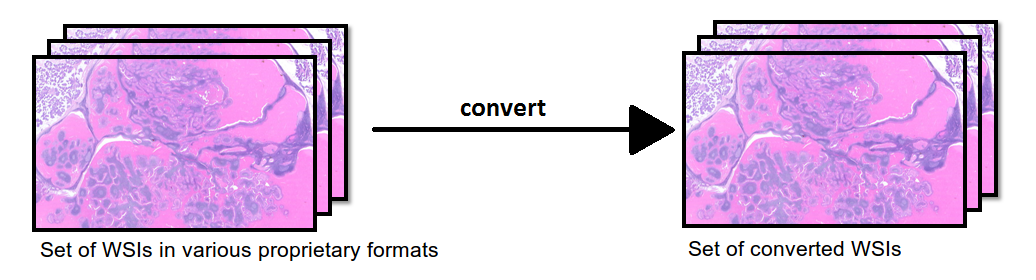
\includegraphics[scale=0.35]{img/processChainA.png}
		\caption{Visualization of the Conversion Service}
		\label{fig:fig2.3}
	\end{center}
\end{figure}

The Conversion Service will be implemented as a python script, which upon calling takes every single WSI of a certain format inside a given folder and converts it to the dzi format. Each converted WSI will be saved in another specified folder. Valid image formats (and their corresponding producers) for conversion are:

\begin{itemize}
	\item .bif (Ventana)
	\item .mrxs (Mirax)
	\item .ndpi (Hamamatsu)
	\item .scn (Leica)
	\item .svs (Aperio)
	\item .svslide (Sakura)
	\item .tif (Aperio, Trestle, Ventana)
	\item .tiff (Philips)
	\item .vms (Hamamatsu)
	\item .vmu (Hamamatsu)
\end{itemize}


\subsection{Annotation Service}

The first step to create a valid training sample for a NN is to annotate the WSIs which will later serve as that. To do so, a GUI\nmc{GUI}{Graphical User Interface} must be deployed which enables a pathologist to make annotations to an WSI. Additionally, the Annotation Service also needs to be capable to persist made annotations (see fig. 2.4). This will happen by saving the annotations into a file which will be placed next to the image.

\begin{figure}[H]
	\begin{center}
		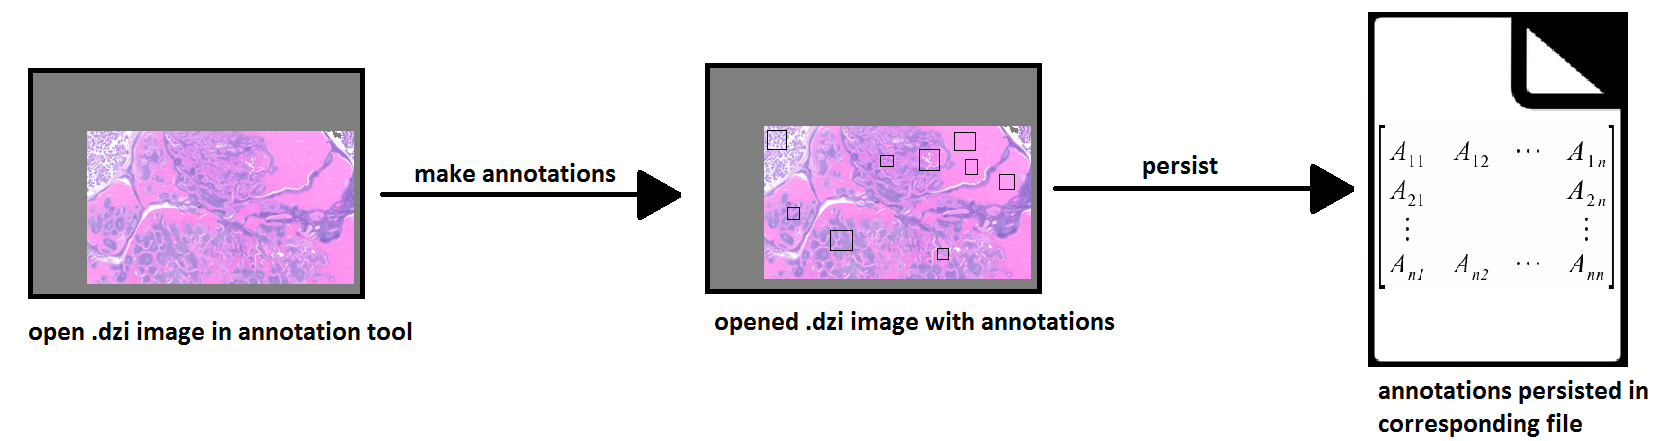
\includegraphics[scale=0.25]{img/processChainB.png}
		\caption{Visualization of the Annotation Service}
		\label{fig:fig2.4}
	\end{center}
\end{figure}

To enable the pathologist to make annotations in the first place, a GUI needs to be offered by the service. This GUI will be developed in iterations with the help of a number of pathologists to adapt it to their wishes and grant the best possible usability. The basic concept of the first iteration will be based on the Microdraw\footnote{See \url{https://github.com/r03ert0/microdraw} for more information on the Microdraw project} GUI (see fig. 2.5).

\begin{figure}[H]
	\begin{center}
		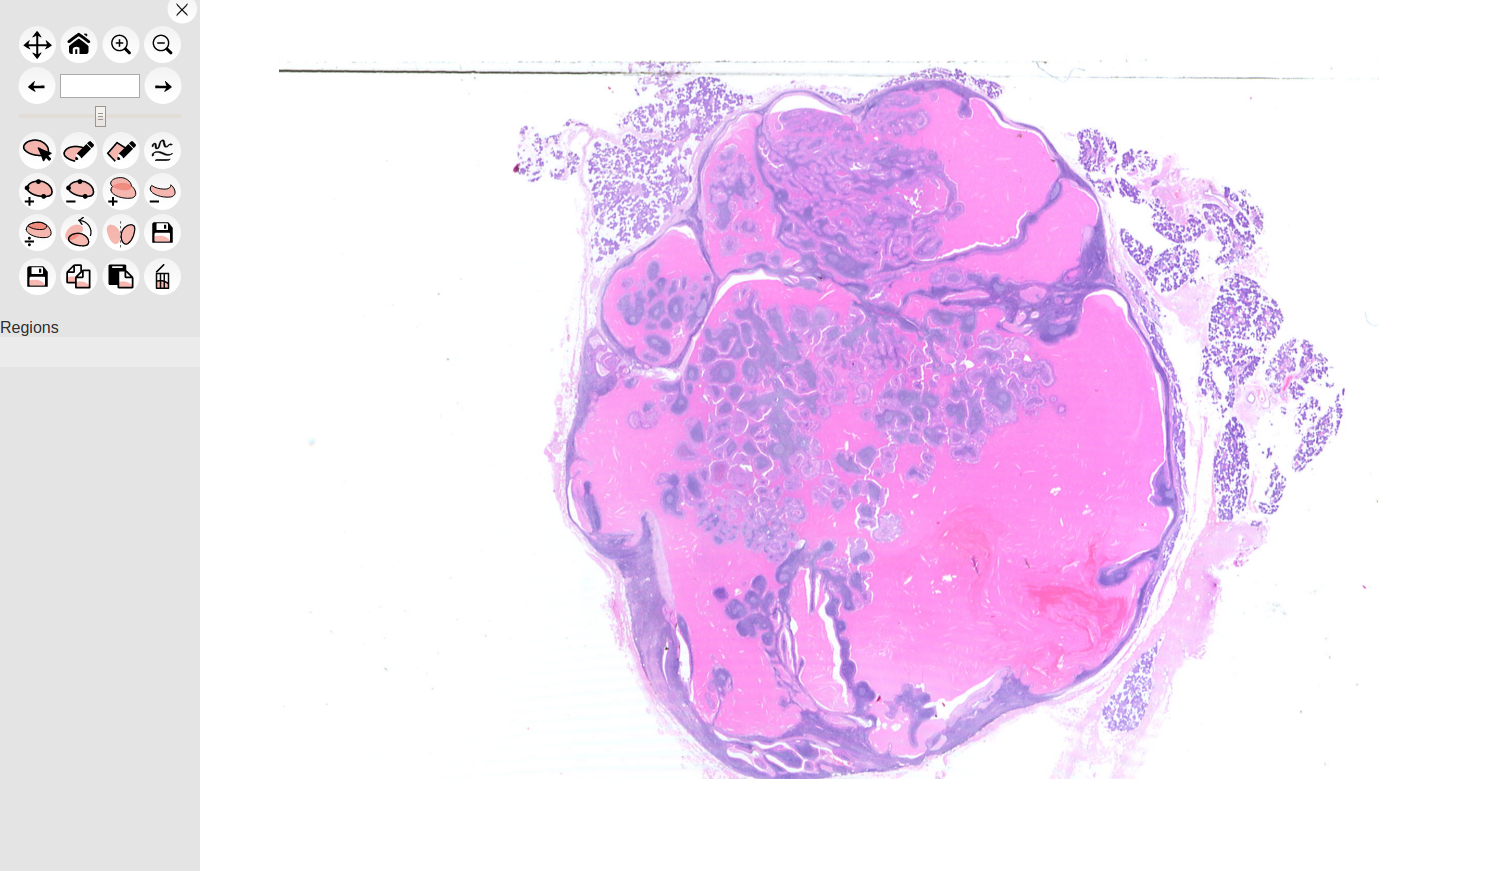
\includegraphics[scale=0.2]{img/microdrawUI.png}
		\caption{Microdraw GUI with opened WSI}
		\label{fig:fig2.5}
	\end{center}
\end{figure}

Microdraw is a webbased annotation tool, which describes itself as

\begin{quotation}
	"[...] a collaborative vectorial annotation tool for ultra high resolution data, such as that produced by high-throughput histology." \cite{web:microdraw}
\end{quotation}

Therefore, the GUI of the Annotation Service, or Annotation Service Viewer (ASV)\nmc{ASV}{Annotation Service Viewer}, will run as a web application in a browser. Annotations will be made by selecting a shape or annotation method from the various tools in the toolbar (see the gray bar on the left in fig. 2.5). After selecting the area to be annotated, an actual description of that area can be made via keyboard input.

When the pathologist is done or wants to save the made annotations, the Annotation Service will create a file in which they will be persisted in. Only one WSI can be opened in one ASV at a time.


\subsection{Tessellation Service}

The task of the Tessellation Service is to tessellate a given WSI into multiple tiles while keeping up the correspondence between image areas and annotations (see fig. 2.6). Tessellation describes the process of seperating a geometric space (e.g. a plane) into multiple tiles of one or more shapes. No matter if the tiles are unifrom or of different shapes, there must be no gaps or overlapping areas in the resulting tiles.

\begin{figure}[H]
	\begin{center}
		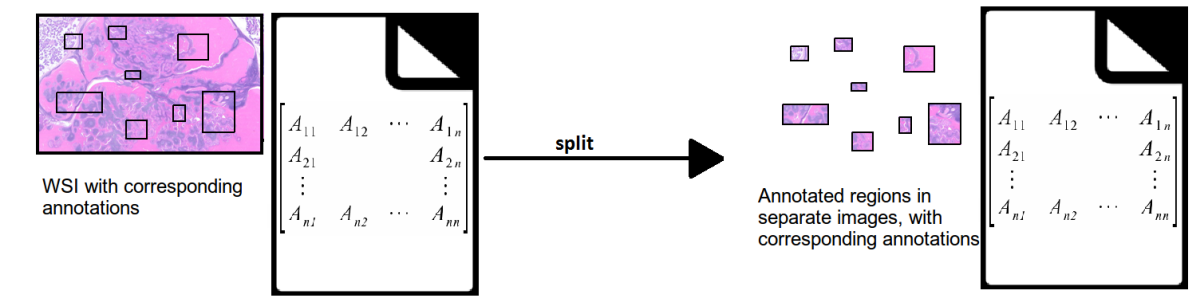
\includegraphics[scale=0.3]{img/processChainC.png}
		\caption{Visualization of the Tessellation Service}
		\label{fig:fig2.6}
	\end{center}
\end{figure}

The tessellation of the Tessellation Service differs from the given definition in two aspects. First, all tiles will be of a unifrom shape (square). Second, the service will also offer the possibility of seperating only the annotated areas of an WSI into tiles. Therefore, the "no gaps" rule is invalid, when this option is chosen. The rule of no overlapping areas holds true in either case, however.

As mentioned before, the second task of the Tessellation Service is to ensure the correspondence between tiles and annotations of the original WSI. This means that, if the original WSI has an annotation in the area of a tile, this tile needs to have the same annotation.

\section{Definition of terms}
To prevent missunderstandings and confusion, the following subsections 2.1.1 - 2.1.3 will define some terminoligy which will be mandatory for the understanding of certain areas of this thesis.


\subsection{Deep Zoom Image Format}

\begin{figure}[H]
	\begin{center}
		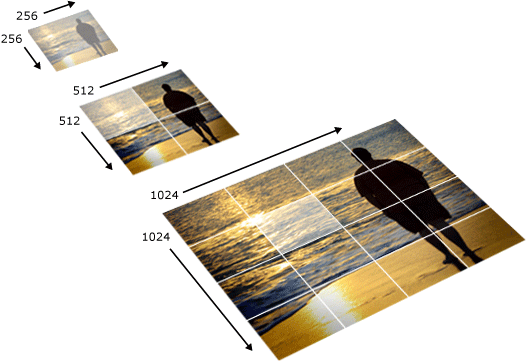
\includegraphics[scale=0.5]{img/dzi_pyramid.png}
		\caption{3 consecutive levels of a dzi image (source: https://i-msdn.sec.s-msft.com/dynimg/IC141135.png)}
		\label{fig:fig2.1}
	\end{center}
\end{figure}

The Deep Zoom Image Format (dzi)\nomenclature{dzi}{Deep Zoom Image Format} is an xml-based file format maintained by Microsoft to improve performance and quality in the handling of large image files. For this purpose an image is represented in a tiled pyramid (see fig. 2.1).

As seen in fig. 2.1 there are multiple versions of a single image in different resolutions. Each resolution in the pyramid is called a \emph{level}. At each level the image is scaled down by the factor 4 (2 in each dimension). Furthermore, the image gets tiled up into $256^2$ tiles (256 in each dimension)\cite{web:dzi}.

If a viewer wants to view a certain area of the image (e.g. the highlighted tile in the last image in fig. 2.1), only the corresponding tiles need to be loaded. This saves large amounts of bandwidth and memory. The same goes for a viewer, who is zoomed out very far. In such a view the full level of detail isn't needed, so that a version from a lower level can be loaded.

A dzi file consists of two parts: a describing .xml file\footnote{Frameworks like \emph{OpenSeaDragon} also support further formats, such as .json.} and a folder with more subfolder. Each subfolder describes a level and as such contains all the tiles for that particular level.


\subsection{Neural Network}
Artificial neural networks (NN)\nmc{NN}{Neural Networks} are a group of models inspiried by biological neural networks\footnote{For the remainder of this thesis, neural network will always represent the artificial one, unless explicitly stated otherwise.}. In a NN, regardless if artificial or biological, many neurons are interconnected with each other. The construct of interconnected neurons can be seperated into layers, of which there are three kinds:

\begin{itemize}
	\item input layer
	\item hidden layer
	\item output layer
\end{itemize}

\begin{figure}[H]
	\begin{center}
		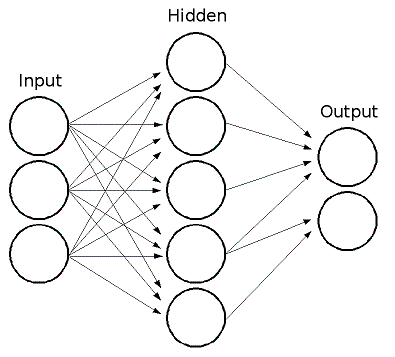
\includegraphics[scale=0.7]{img/mlp.png}
		\caption{3 layer NN (source: http://docs.opencv.org/2.4/\textunderscore images/mlp.png)}
		\label{fig:fig2.2}
	\end{center}
\end{figure}

Basically, the input layer, as the name suggests, is the layer where the NN gets its input data from. After that, there are a number of hidden layers\footnote{A NN doesn't necessarily need to have any hidden layers. For non trivial problems however, it becomes mandatory.}, which are responsible for further computation of the input values. At the end is the output layer which is responsible for communicating the results of the prior operations (compare fig. 2.2). Each single neuron has input values and an output value. Once the input reaches a certain trigger point, the cell in the neuron sends a signal as output. 

A huge benefit of NN, over other software models, is their ability to learn. While certain problems are easier to solve in a sequential, algorithmic fashion (say an equation or the towers of hanoi), certain problems are so complex that new approaches are needed, while other problems can't be solved algorithmic at all. With the use of adequate training samples, a NN can train to solve a problem, not unlike a human, by learning. Since this topic alone is enough for a number of theses, the author refers to \cite{Kriesel07} for further detailed information.
